% Worked Examples: Concept 1.1.4 - Modelling Methodology
\documentclass[11pt,a4paper]{article}
\usepackage{worked-examples-template}

\title{\textbf{Worked Examples}\\[0.5em]
\large Concept 1.1.4: Modelling Methodology\\[0.3em]
\normalsize \coursesubtitle{} -- \coursetitle}
\author{Assoc.\ Prof.\ William Robertson \and Dr Sean McGowan}
\date{\today}

\begin{document}

\maketitle
\tableofcontents
\newpage

\section{Concept 1.1.4: Modelling}

\subsection{Example 1: Free Falling Skydiver with Nonlinear Drag}

\paragraph{Problem:} A skydiver of mass $m = 80$ kg jumps from an aircraft. Model the vertical motion of the skydiver considering gravitational force and nonlinear air drag. The drag force is proportional to the square of velocity: $F_d = \frac{1}{2}\rho C_d A v^2$, where $\rho = 1.2$ kg/m$^3$ is air density, $C_d = 1.0$ is the drag coefficient, and $A = 0.5$ m$^2$ is the cross-sectional area.

\begin{figure}[h]
\centering
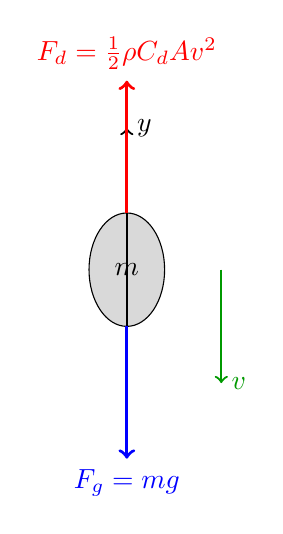
\begin{tikzpicture}[scale=1.2]
  % Draw the skydiver (simplified)
  \draw[fill=gray!30] (0,0) ellipse (0.4 and 0.6);
  \node at (0,0) {$m$};
  
  % Coordinate system
  \draw[->,thick] (0,-1.5) -- (0,1.5) node[right] {$y$};
  
  % Forces
  \draw[->,very thick,blue] (0,-0.6) -- (0,-2) node[below] {$F_g = mg$};
  \draw[->,very thick,red] (0,0.6) -- (0,2) node[above] {$F_d = \frac{1}{2}\rho C_d A v^2$};
  
  % Velocity arrow
  \draw[->,thick,green!60!black] (1,0) -- (1,-1.2) node[right] {$v$};
  
\end{tikzpicture}
\caption{Free body diagram of a falling skydiver with forces acting on the body.}
\end{figure}

\paragraph{Solution:} 

Applying Newton's second law in the vertical direction (taking downward as positive):
\begin{align}
m\frac{dv}{dt} &= mg - \frac{1}{2}\rho C_d A v^2
\end{align}

This can be rewritten as:
\begin{align}
\frac{dv}{dt} &= g - \frac{\rho C_d A}{2m} v^2
\end{align}

Let $k = \frac{\rho C_d A}{2m}$, then:
\begin{align}
\frac{dv}{dt} &= g - kv^2
\end{align}

Substituting the given values:
\begin{align}
k &= \frac{1.2 \times 1.0 \times 0.5}{2 \times 80} = 0.00375 \text{ m}^{-1}
\end{align}

The terminal velocity occurs when $\frac{dv}{dt} = 0$:
\begin{align}
v_{\text{terminal}} &= \sqrt{\frac{g}{k}} = \sqrt{\frac{9.81}{0.00375}} \approx 51.1 \text{ m/s}
\end{align}

The state-space model is:
\begin{align}
\frac{dv}{dt} &= 9.81 - 0.00375v^2 \\
\frac{dy}{dt} &= v
\end{align}

This is a nonlinear first-order differential equation in $v$ and can be solved numerically or analytically using separation of variables.

\subsection{Example 2: Flow Rate and Temperature in a Pipe}

\paragraph{Problem:} Consider a heated pipe system where fluid flows at rate $q$ (m$^3$/s) through a pipe of volume $V = 0.1$ m$^3$. The fluid enters at temperature $T_{\text{in}}$ and is heated by a heater providing power $P$ (W). Model the outlet temperature $T$ considering heat input and convective flow. The fluid has density $\rho = 1000$ kg/m$^3$ and specific heat capacity $c_p = 4200$ J/(kg·K).

\begin{figure}[h]
\centering
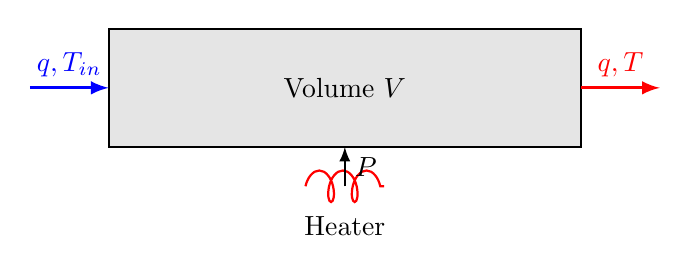
\begin{tikzpicture}[>=latex]
  % Pipe
  \draw[thick,fill=gray!20] (0,0) rectangle (6,1.5);
  \node at (3,0.75) {Volume $V$};
  
  % Inlet
  \draw[->,very thick,blue] (-1,0.75) -- (0,0.75) node[midway,above] {$q, T_{\text{in}}$};
  
  % Outlet
  \draw[->,very thick,red] (6,0.75) -- (7,0.75) node[midway,above] {$q, T$};
  
  % Heater
  \draw[thick,red,decorate,decoration={coil,aspect=0.5,segment length=3mm,amplitude=2mm}] 
    (2.5,-0.5) -- (3.5,-0.5);
  \draw[->,thick] (3,-0.5) -- (3,0) node[midway,right] {$P$};
  \node at (3,-1) {Heater};
  
\end{tikzpicture}
\caption{Schematic of a heated pipe system with flow rate and temperature dynamics.}
\end{figure}

\paragraph{Solution:}

Energy balance for the fluid in the pipe:
\begin{align}
\frac{d}{dt}(\rho V c_p T) &= \rho q c_p T_{\text{in}} - \rho q c_p T + P
\end{align}

Assuming constant volume and properties:
\begin{align}
\rho V c_p \frac{dT}{dt} &= \rho q c_p (T_{\text{in}} - T) + P
\end{align}

Dividing by $\rho V c_p$:
\begin{align}
\frac{dT}{dt} &= \frac{q}{V}(T_{\text{in}} - T) + \frac{P}{\rho V c_p}
\end{align}

Let $\tau = \frac{V}{q}$ be the residence time, then:
\begin{align}
\frac{dT}{dt} &= \frac{1}{\tau}(T_{\text{in}} - T) + \frac{P}{\rho V c_p}
\end{align}

For $q = 0.01$ m$^3$/s:
\begin{align}
\tau &= \frac{0.1}{0.01} = 10 \text{ s}
\end{align}

The state-space model is:
\begin{align}
\frac{dT}{dt} &= 0.1(T_{\text{in}} - T) + \frac{P}{420000}
\end{align}

This is a first-order linear system with two inputs ($T_{\text{in}}$ and $P$) and one state ($T$).

At steady state ($\frac{dT}{dt} = 0$):
\begin{align}
T_{\text{ss}} &= T_{\text{in}} + \frac{P}{\rho q c_p}
\end{align}

\subsection{Example 3: Predator-Prey Population Dynamics (Foxes and Rabbits)}

\paragraph{Problem:} Model the population dynamics of rabbits (prey) and foxes (predators) in an ecosystem. Let $R(t)$ be the rabbit population and $F(t)$ be the fox population. Use the Lotka-Volterra model with the following assumptions:
\begin{itemize}
\item Rabbits reproduce at rate $\alpha = 0.1$ per month in the absence of predators
\item Foxes prey on rabbits at rate $\beta = 0.02$ per month per rabbit
\item Foxes die at rate $\gamma = 0.4$ per month without food
\item Fox population grows at rate $\delta = 0.01$ per rabbit consumed
\end{itemize}

\begin{figure}[h]
\centering
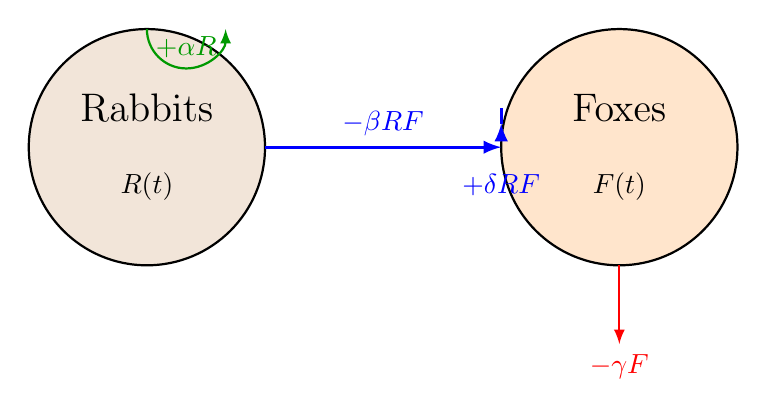
\begin{tikzpicture}[>=latex]
  % Rabbits
  \draw[thick,fill=brown!20] (0,0) circle (1.5);
  \node at (0,0.5) {\Large Rabbits};
  \node at (0,-0.5) {$R(t)$};
  
  % Foxes
  \draw[thick,fill=orange!20] (6,0) circle (1.5);
  \node at (6,0.5) {\Large Foxes};
  \node at (6,-0.5) {$F(t)$};
  
  % Birth rate (rabbits)
  \draw[->,thick,green!60!black] (0,1.5) arc (180:360:0.5) node[midway,above] {$+\alpha R$};
  
  % Death rate (foxes)
  \draw[->,thick,red] (6,-1.5) -- (6,-2.5) node[below] {$-\gamma F$};
  
  % Predation
  \draw[->,very thick,blue] (1.5,0) -- (4.5,0) node[midway,above] {$-\beta RF$};
  \draw[->,very thick,blue] (4.5,0.3) -- (4.5,0.3) node[midway,below,yshift=-5mm] {$+\delta RF$};
  
\end{tikzpicture}
\caption{Population dynamics showing interaction between rabbits (prey) and foxes (predators).}
\end{figure}

\paragraph{Solution:}

The Lotka-Volterra equations are:
\begin{align}
\frac{dR}{dt} &= \alpha R - \beta RF \\
\frac{dF}{dt} &= -\gamma F + \delta RF
\end{align}

Substituting the given parameters:
\begin{align}
\frac{dR}{dt} &= 0.1R - 0.02RF \\
\frac{dF}{dt} &= -0.4F + 0.01RF
\end{align}

This is a nonlinear system with two state variables $(R, F)$.

Equilibrium points occur when $\frac{dR}{dt} = \frac{dF}{dt} = 0$:

\textbf{Equilibrium 1:} $R = 0, F = 0$ (extinction)

\textbf{Equilibrium 2:} Setting both derivatives to zero:
\begin{align}
0.1R - 0.02RF &= 0 \quad \Rightarrow \quad R(0.1 - 0.02F) = 0 \\
-0.4F + 0.01RF &= 0 \quad \Rightarrow \quad F(-0.4 + 0.01R) = 0
\end{align}

For non-trivial solution:
\begin{align}
0.1 - 0.02F &= 0 \quad \Rightarrow \quad F^* = 5 \\
-0.4 + 0.01R &= 0 \quad \Rightarrow \quad R^* = 40
\end{align}

The equilibrium point is $(R^*, F^*) = (40, 5)$. This system exhibits periodic oscillations around this equilibrium, characteristic of predator-prey dynamics.

\subsection{Example 4: Operational Amplifier Inverting Configuration}

\paragraph{Problem:} Model an operational amplifier in the inverting configuration with input resistance $R_1 = 10$ k$\Omega$ and feedback resistance $R_f = 100$ k$\Omega$. Assume the op-amp has finite open-loop gain $A = 10^5$ and a single-pole frequency response with bandwidth $\omega_0 = 10$ rad/s. Derive the closed-loop transfer function.

\begin{figure}[h]
\centering
\begin{circuitikz}[scale=1.0]
  % Op-amp
  \draw (0,0) node[op amp] (opamp) {};
  
  % Input resistor
  \draw (-4,0.5) to[R=$R_1$,o-] (-2,0.5) -- (opamp.-);
  \node at (-4.5,0.5) {$v_{\text{in}}$};
  
  % Feedback resistor
  \draw (opamp.-) -- (-2,0.5) to[R=$R_f$] (-2,3) -- (2,3) -- (2,0) -- (opamp.out);
  
  % Ground connection
  \draw (opamp.+) -- (-2,-0.5) node[ground] {};
  
  % Output
  \draw (opamp.out) to[short,-o] (3,0) node[right] {$v_{\text{out}}$};
  
  % Virtual ground label
  \node at (-2.5,0.5) [above] {$v_n$};
  
\end{circuitikz}
\caption{Inverting operational amplifier configuration with input and feedback resistors.}
\end{figure}

\paragraph{Solution:}

For an ideal op-amp with finite gain $A$:
\begin{align}
v_{\text{out}} &= -A v_n
\end{align}

where $v_n$ is the voltage at the inverting input (node voltage).

Applying Kirchhoff's current law at the inverting input node:
\begin{align}
\frac{v_{\text{in}} - v_n}{R_1} + \frac{v_{\text{out}} - v_n}{R_f} &= 0
\end{align}

Substituting $v_{\text{out}} = -Av_n$:
\begin{align}
\frac{v_{\text{in}} - v_n}{R_1} + \frac{-Av_n - v_n}{R_f} &= 0
\end{align}

Solving for $v_n$:
\begin{align}
v_{\text{in}} - v_n + \frac{R_1}{R_f}(-Av_n - v_n) &= 0 \\
v_{\text{in}} &= v_n\left(1 + \frac{R_1}{R_f}(A + 1)\right) \\
v_n &= \frac{v_{\text{in}}}{1 + \frac{R_1}{R_f}(A + 1)}
\end{align}

The closed-loop gain is:
\begin{align}
\frac{v_{\text{out}}}{v_{\text{in}}} &= \frac{-Av_n}{v_{\text{in}}} = \frac{-A}{1 + \frac{R_1}{R_f}(A + 1)}
\end{align}

For large $A$, this simplifies to:
\begin{align}
\frac{v_{\text{out}}}{v_{\text{in}}} &\approx \frac{-A}{\frac{R_1}{R_f}A} = -\frac{R_f}{R_1}
\end{align}

With $R_1 = 10$ k$\Omega$ and $R_f = 100$ k$\Omega$:
\begin{align}
\frac{v_{\text{out}}}{v_{\text{in}}} &\approx -10
\end{align}

For frequency response with single-pole dynamics, let $A(s) = \frac{A_0}{1 + s/\omega_0}$:
\begin{align}
\frac{v_{\text{out}}(s)}{v_{\text{in}}(s)} &= \frac{-R_f/R_1}{1 + \frac{1 + R_f/R_1}{A_0}(1 + s/\omega_0)}
\end{align}

This shows that the op-amp circuit acts as an inverting amplifier with gain determined primarily by the resistor ratio, with finite bandwidth effects from the op-amp's frequency response.
\end{document}
